\section{Find SRLG Conflicting Link Set}
\label{sec:Find SRLG conflict link set}
In this section, we describe how to find a SRLG Conflicting Link Set for a given AP for which there is no SRLG-disjoint BP in a network $G$.

\subsection{Build a new graph $G^*$ with novel link capability setting principle}

As introduced in Section \ref{sec:PRELIMINARIES},  if all the links in the cut-set $\mathbb{\mathbb{L}}_{\Phi}$ are removed in a graph $G$, then $|f| = 0$. That is, no flow can pass from $s$ to $d$. In this paper,  we try to find the SRLG Conflicting Link Set based on the concept of the cut-set. If an AP flow passes from $s$ to $d$ through a path that shares the risk with  all links in the cut-set, then no SRLG-disjoint BP can be found, as no link in the cut-set can be selected for a BP path to pass through the cut.

To facilitate finding the SRLG Conflicting Link Set based on the cut-set, we construct a new graph $G^*$ as follows.

1) $G^*$ uses the same ${\mathbb{V}}$ and ${\mathbb{E}}$ of $G$.

2) The link weight $w_{e_i}$ associated with each link $e_i \in \mathbb{E}$ is the same as the corresponding link weight of graph $G$.

3) We adopt the following principle to set the capacity $c_{e_i}$ associated with each link $e_i \in \mathbb{E}$:
  \begin{equation}
c_{e_i} = \left\{ {\begin{array}{*{20}{c}}
   1 & {e_i{\rm{ }} \in {\rm{ \mathbb{AP}}}}  \\
   {\left| \mathbb{AP} \right|+1} & {e_i{\rm{ }} \in {\rm{ \mathbb{E}}}{{\rm{\mathbb{R}}}}}  \\
   {\left| {{\rm\mathbb{AP}}} \right| + \left( {\left| {{\rm\mathbb{AP}}} \right| + 1} \right)\times \left| {{\rm{\mathbb{E}}}{{\rm{\mathbb{R}}}}} \right| + 1} & {otherwise}  \\
\end{array}} \right.
\label{eq:capacity principle}
\end{equation}
where $\mathbb{AP}$ denotes the set of links forming the smallest weight path $AP$ in the graph $G$,  and $\mathbb{\mathbb{ER}}$ denotes the set of links not belonging to AP that share the common risks with AP.

In Fig.\ref{fig:CompositeGraph}(c), the link set of  AP is $\mathbb{AP}=\{e_1,e_2,e_3,e_4$
$,e_5,e_6,e_7,e_8\}$, $\mathbb{\mathbb{ER}}=\{e_9,e_{11},e_{17},e_{13},e_{19}\}$. We have $|\mathbb{AP}|=8$, $|\mathbb{\mathbb{ER}}|=5$, $|\mathbb{AP}|+1=9$ and ${\left| {{\rm{\mathbb{AP}}}} \right| + \left( {\left| {{\rm{\mathbb{AP}}}} \right| + 1} \right)\times \left| {{\rm{\mathbb{E}}}{{\rm{\mathbb{R}}}}} \right| + 1}=54$. We generate a new graph $G^*$ in Fig.\ref{fig:FlowStarGraph}, with the capacity of the links set in the graph $G^*$   according to the principle in Equ.(\ref{eq:capacity principle}).

In Section \ref{subsec:Properties on the min-cut in the new graph $G^*$}, we will demonstrate that when an AP encounters the trap problem, such principles make the min cut-set in the new graph  belonging either to $\mathbb{AP}$ or $\mathbb{\mathbb{ER}}$, which further provides the possibility of obtaining the SRLG Conflicting Link Set with the links on the AP.

%According to the principle defined in (\ref{eq:capacity principle}), we set the capacity of the links in the graph. Given the network in Fig.\ref{fig:Initial Graph}, as $\mathbb{AP}=\{e_1,e_2,e_3,e_4,e_5,e_6,e_7,e_8\}$ and $\mathbb{\mathbb{ER}}=\{e_9,e_{11},e_{17},e_{13},e_{19}\}$, we have $|\mathbb{AP}|=8$, $|\mathbb{\mathbb{ER}}|=5$, $|\mathbb{AP}|+1=9$ and ${\left| {{\rm{\mathbb{AP}}}} \right| + \left( {\left| {{\rm{\mathbb{AP}}}} \right| + 1} \right)\times \left| {{\rm{\mathbb{E}}}{{\rm{\mathbb{R}}}}} \right| + 1}=55$. Therefore, the new graph with capacity being set following the principle in (\ref{eq:capacity principle}) is shown in Fig.\ref{fig:FlowStarGraph}.

\begin{figure}[tp]
  \centering
  % Requires \usepackage{graphicx}
  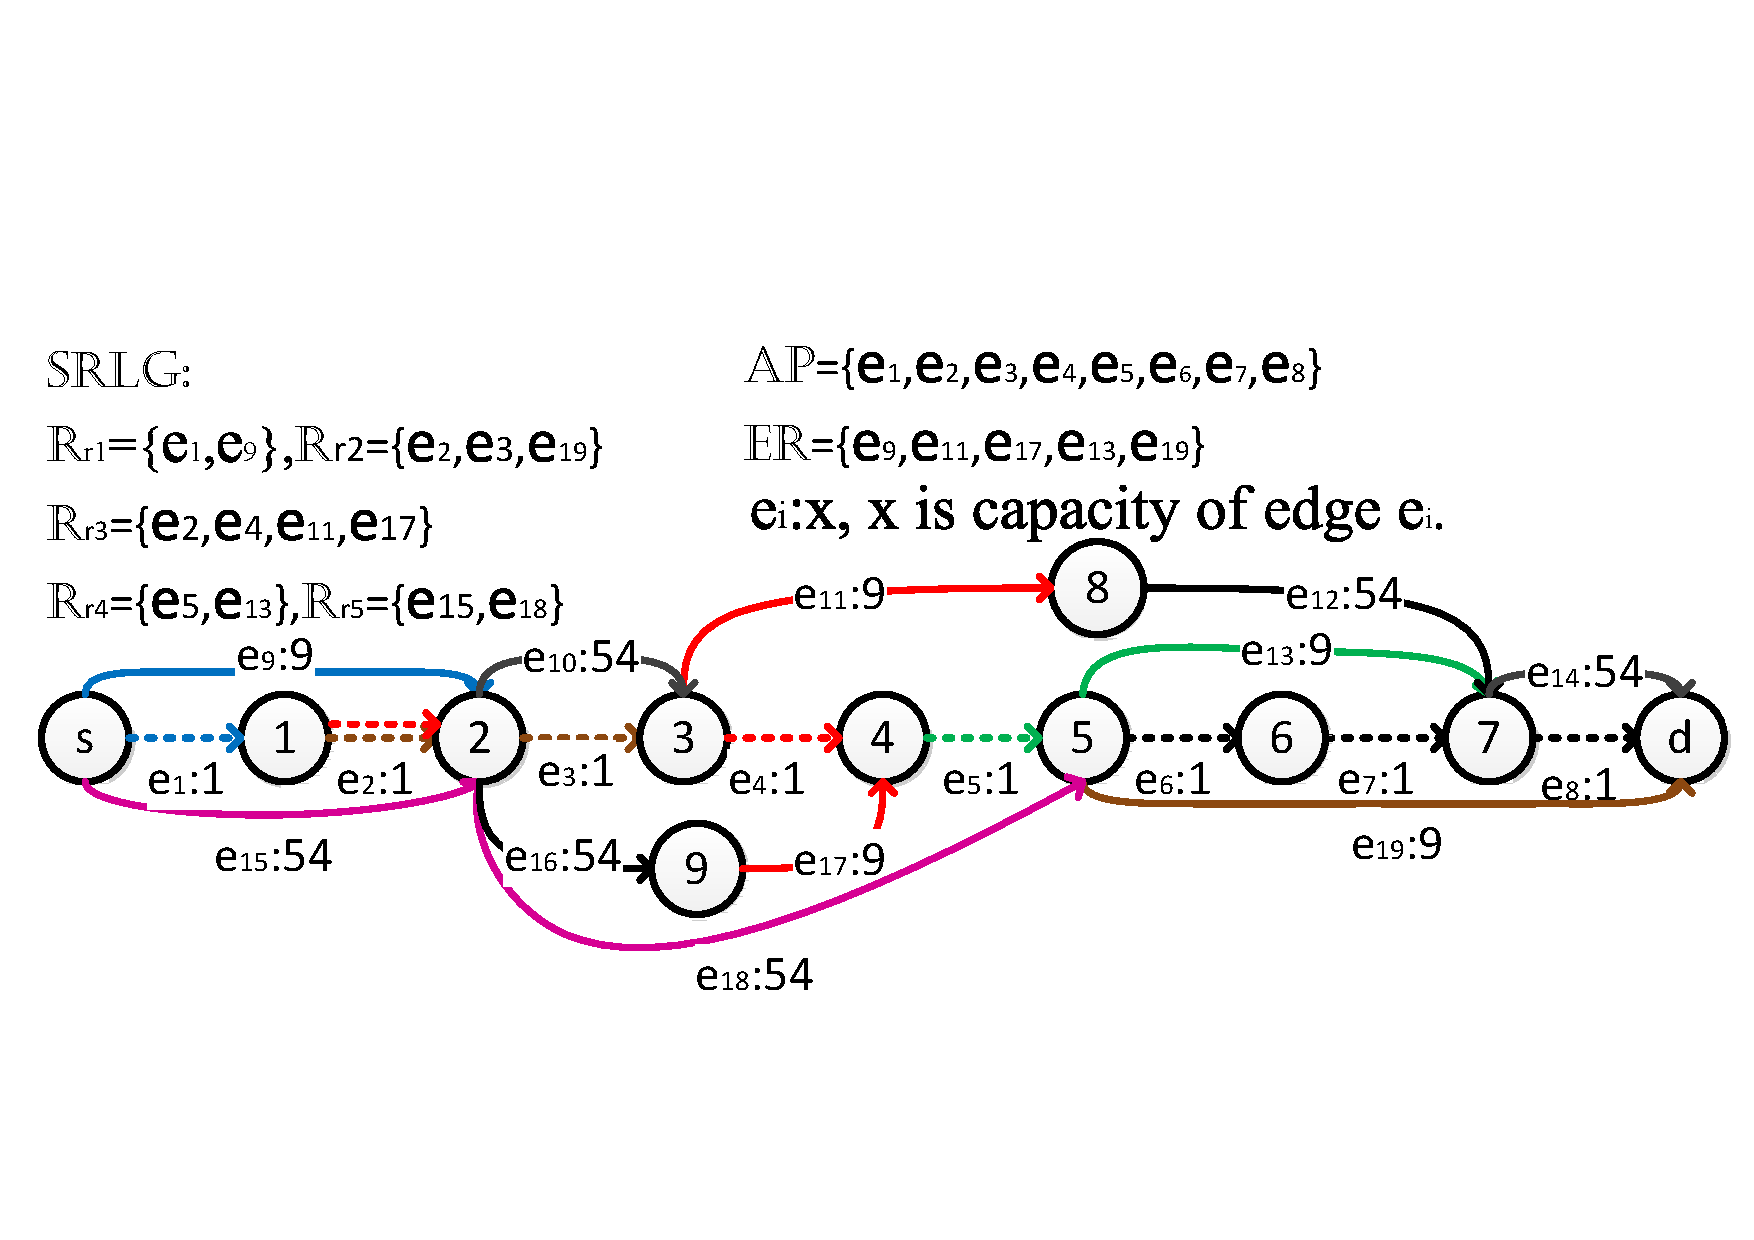
\includegraphics[width=3.6in]{franz/FlowStarGraph}
  \caption{New Graph $G^*$}\label{fig:FlowStarGraph}
\end{figure}
\subsection{Properties on the min-cut in the new graph $G^*$}
\label{subsec:Properties on the min-cut in the new graph $G^*$}
The max-flow min-cut theorem states that in a  network the maximum amount of flow passing from the source $s$ to the destination $d$ is equal to the total capacity of the links in the minimum cut, i.e. the smallest total capacity of the links which if removed would disconnect the destination $d$ from the source $s$.  Our algorithm will find the minimum SRLG Conflicting Link Set based on the min-cut of the graph.

We will first show that some good properties of our rebuilt graph $G^*$ can serve as a base to find the minimum SRLG Conflicting Link Set.


Let $\Phi$=${(\mathbb{S}},{\mathbb{D}})$ be a min-cut of $G^*$ and $\mathbb{L}_{\Phi}$  represent the \textbf{cut-set}. Fig.\ref{fig:MinCutStarGraph} shows the min-cut $\Phi$=${(\mathbb{S}},{\mathbb{D}})$ with ${\mathbb{S}}=\{s, 1, 2, 3, 4, 5, 9\}$,  ${\mathbb{D}}=\{6, 7, 8, d\}$, and $\mathbb{L}_{\Phi}=\{e_{11}, e_{13}, e_{19}, e_6\}$.


\begin{lemma}
\label{le:lemma1}
    Any path from $s$ to $d$ in $G^*$ must pass through at least one link in $\mathbb{AP}$ or $\mathbb{\mathbb{ER}}$.
    %note:draw a picture to describe the proof
\end{lemma}
\begin{proof}
We prove the lemma by the way of contradiction. Assume that for the AP, there exists another path from  $s$ to $d$ in $G^*$ that does not share the risks with  AP, that is, the path does not pass through the links in $\mathbb{AP}$ or $\mathbb{\mathbb{ER}}$. We can easily conclude that this path is the SRLG-disjoint BP for the AP, which contradicts with the claim that there is no SRLG-disjoint BP for the AP in the network.
\end{proof}

\begin{lemma}
\label{le:lemma2}
    The value of any max flow from s to d in $G^*$ is at most $|\mathbb{AP}|+(|\mathbb{AP}|+1)\times|\mathbb{\mathbb{ER}}|$.
\end{lemma}
\begin{proof}
Assume the value of a max flow $f$ of $G^*$ is $|f|=k$. $f$ can be  partitioned into $k$ 1-unit-flows from $s$ to $d$ in  $G^*$.
According to Lemma.\ref{le:lemma1}, each of these 1-unit-flows must pass through at least one link in $\mathbb{AP}$ or $\mathbb{\mathbb{ER}}$.
 Note that the capacity of the links in  $\mathbb{AP}$ or $\mathbb{\mathbb{ER}}$ are in $1$ and $|\mathbb{AP}|$+1, respectively. According to the capacity set for the links in $\mathbb{AP}$ and $\mathbb{\mathbb{ER}}$, a link in $\mathbb{AP}$ can carry only one unit-flow traffic, while the  link in $\mathbb{ER}$ can be shared by at most  $|\mathbb{AP}|$+1 unit-flows.
 Therefore, there can be at most $|\mathbb{AP}|+ (|\mathbb{AP}|+1)\times|\mathbb{\mathbb{ER}}|$ such unit-flows from s to d.
\end{proof}

\begin{lemma}
\label{le:lemma3}
    All  links in the \textbf{cut-set} $\mathbb{L}_{\Phi}$ of the min-cut $\Phi$ of $G^*$ belong to $\mathbb{AP}$ or $\mathbb{\mathbb{ER}}$.
\end{lemma}
\begin{proof}
    According to the max-flow min-cut theorem, the capacity of the min-cut $\Phi$, denoted by $c(\Phi)$, should be equal to the max-flow value, which is at most $|\mathbb{AP}|+ |\mathbb{ER}|\times (|\mathbb{AP}|+1)$ according to lemma.\ref{le:lemma2}. According to the capacity setting principle defined in Eq.(\ref{eq:capacity principle}), for the links that are neither in $\mathbb{AP}$ nor in $\mathbb{ER}$ (that is $e_i \notin \mathbb{AP}$ and $e_i \notin \mathbb{ER}$), their capacity is $c_{e_i} = \left| {{\rm\mathbb{AP}}} \right| + \left( {\left| {{\rm\mathbb{AP}}} \right| + 1} \right)\times \left| {{\rm{\mathbb{E}}}{{\rm{\mathbb{R}}}}} \right| + 1$, which is larger than $|\mathbb{AP}|+(|\mathbb{AP}|+1)\times |\mathbb{ER}|$. Thus, none of them can be a link in the \textbf{cut-set} $\mathbb{L}_{\Phi}$. So all the  links in the \textbf{cut-set} $\mathbb{L}_{\Phi}$ must belong to $\mathbb{AP}$ or $\mathbb{ER}$.
\end{proof}
In the network with SRLG, if  a link is selected by an AP or shares the same risk with the links selected in the AP, this link can not be selected as the SRLG-disjoint BP of the AP. We call this link "blocked" by the AP.

\begin{theorem}
    If a path of a unit-flow of $G$ blocks all the links in \textbf{cut-set} $\mathbb{L}_{\Phi}$, then no more flow can pass through the cut of the graph.
\label{th:block flow}
\end{theorem}

\begin{proof}
    If a path of a unit-flow blocks all the links in \textbf{cut-set} $\mathbb{L}_{\Phi}$, then no flow can use the links in  $\mathbb{L}_{\Phi}$ and thus no more flow can pass the cut $\Phi$.
\end{proof}

Theorem \ref{th:block flow} provides us the possibility to find the SRLG Conflicting Link Set. That is, when an AP encounters a trap problem, we can find the sub-set of \del{the} $\mathbb{AP}$  that can block all the links in \rev{the} \textbf{cut-set} $\mathbb{L}_{\Phi}$, and this sub-set of links can form the  SRLG Conflicting Link Set. When any a path contains all links in the SRLG Conflicting Link Set, no more flow can pass the cut $\Phi$, thus no SRLG-disjoint BP can be found.


\subsection{Set cover problem for SRLG Conflicting Link Set}
\label{subsec:Set cover problem for SRLG Conflicting Link Set}
Although together all links on the AP path form a SRLG Conflicting Link Set, we are interested in a set that has as few links as possible, as the size of the SRLG Conflicting Link Set determines the number of sub-problems partitioned according to Section \ref{subsec:dividedconquer}.


According to theorem \ref{th:block flow}, \textbf{the minimum SRLG Conflicting Link Set finding problem} can be described as:  find the minimum subset of links on AP  that can block all the  links in the \textbf{cut-set} $\mathbb{L}_{\Phi}$.

For any link $e_i$, let $\mathbb{SR}_{e_i}$ denote the link set that shares risks with $e_i$. Obviously, $\mathbb{SR}_{e_i}$ covers $e_i$ itself and all the links in the SRLG that includes $e_i$. For example in Fig.\ref{fig:MinCutStarGraph}, as $e_2$ is in two SRLGs $\mathbb{R}_{r_2}=\{e_2,e_3,e_{19}\}$, $\mathbb{R}_{r_3}=\{e_2,e_4,e_{11},e_{17}\}$, therefore, $\mathbb{SR}_{e_2}=\{e_2,e_3,e_{19},e_4,e_{11},e_{17}\}$.

For each link $e_i$ on AP, we define its cut-block-link set as ${\mathbb{B}_{{e_i}}} = \mathbb{SR}_{{e_i}} \cap \mathbb{L}_{\Phi}$, which is the sub-set of \textbf{cut-set} $\mathbb{L}_{\Phi}$ that can be blocked by $e_i$.

Therefore, the minimum SRLG Conflicting Link Set finding problem can be formulated as a Set Cover Problem: given $\mathbb{AP}$ (the link set of path links of $AP$), the \textbf{cut-set} $\mathbb{L}_{\Phi}$,  and a collection of the cut-block-link sets ${\mathbb{B}_{{e_1}}},{\mathbb{B}_{{e_2}}}, \cdots ,{\mathbb{B}_{{e_{|\mathbb{AP}|}}}}$, we want to find the fewest sets whose union is $\mathbb{L}_{\Phi}$, that is, the smallest $\mathbb{T} \subseteq \{e_i| e_i\in \mathbb{AP}\}$ such that ${ \cup_{e_i \in \mathbb{T}}}{\mathbb{B}_{e_i}} = \mathbb{L}_{\Phi}$.

\begin{figure}[tp]
  \centering
  % Requires \usepackage{graphicx}
  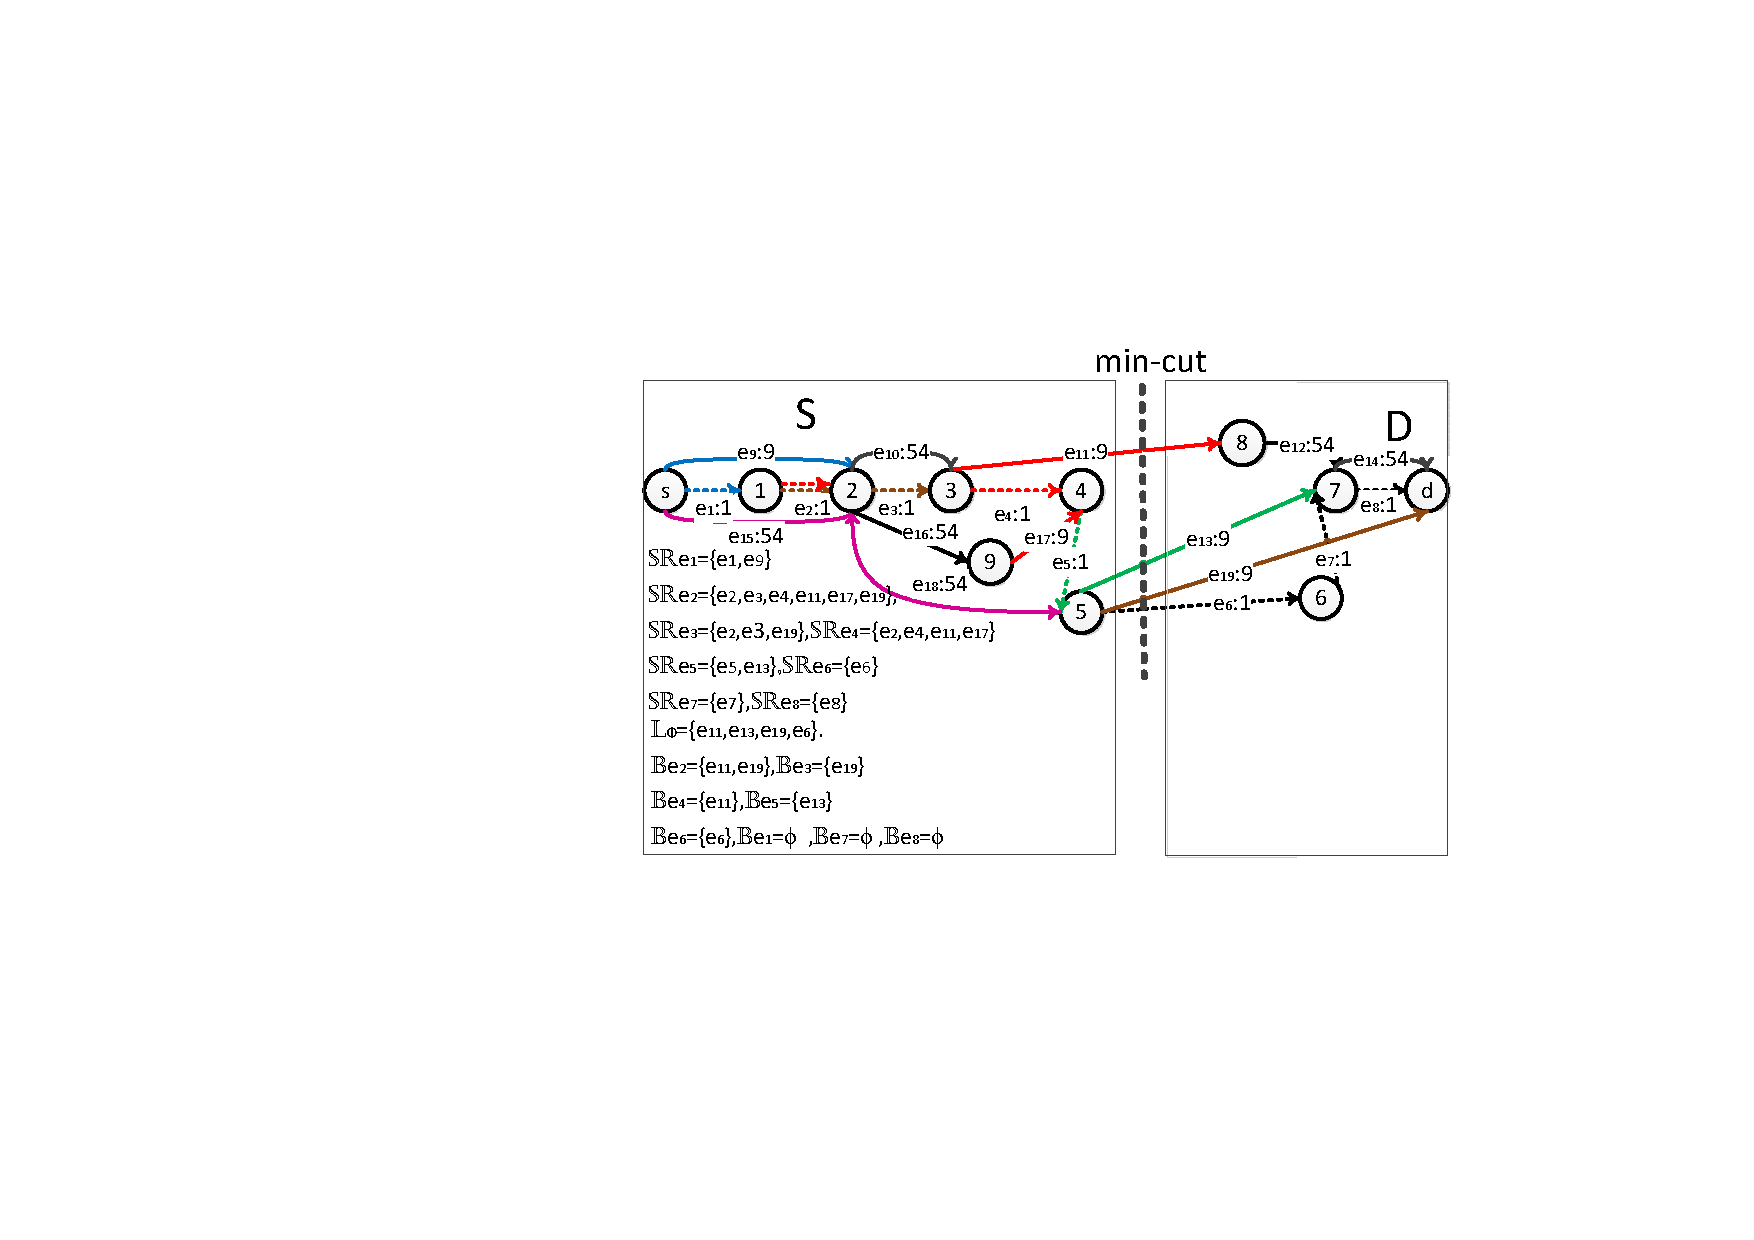
\includegraphics[width=3.6in]{franz/MinCutStarGraph}
  \caption{Min cut of the network graph, $\mathbb{SR}_{e_1}=\{e_1, e_9\},\mathbb{SR}_{e_2}=\{e_2,e_3,e_4, e_{11},e_{17},e_{19}\},\mathbb{SR}_{e_3}=\{e_2,e_3, e_{19}\},\mathbb{SR}_{e_4}=\{e_2,e_4, e_{11},e_{17}\},\mathbb{SR}_{e_5}=\{e_5, e_{13}\},\mathbb{SR}_{e_6}=\{e_6\},\mathbb{SR}_{e_7}=\{e_7\} $ and $\mathbb{SR}_{e_8}=\{e_8\}$. $\mathbb{L}_{\Phi}=\{e_{11},e_{13},e_{19},e_{6}\}$. $\mathbb{B}_{e_1}=\emptyset,\mathbb{B}_{e_2}=\{e_{11},e_{19}\},\mathbb{B}_{e_3}=\{e_{19}\},\mathbb{B}_{e_4}=\{e_{11}\},\mathbb{B}_{e_5}=\{e_{13}\},\mathbb{B}_{e_6}=\{e_6\}$,$\mathbb{B}_{e_7}=\emptyset$ and $\mathbb{B}_{e_8}=\emptyset$.}\label{fig:MinCutStarGraph}
  \label{fig:MinCutStarGraph}
\end{figure}

The Set Cover Problem is usually an NP-hard problem with its complexity depending on the size of the elements (denoted by $n$). In our minimum SRLG Conflicting Link Set finding problem, $n=|\mathbb{L}_{\Phi}|$, that is, the edge number of cut set $\mathbb{L}_{\Phi}$. As this paper's focus is not to improve the solution of the set cover problem, we apply the algorithm proposed in \cite{chvatal1979greedy} with the complexity $O(log(|\mathbb{L}_{\Phi}|))$  to find the minimum SRLG Conflicting Link Set.

The number of subproblems to partition in our divide-and-conquer algorithm is determined by the size of the SRLG Conflicting Link Set, which is at most \rev{equal to} the hop number of \del{the} AP. The random graph of Erd{\"o}s, and R{\'e}nyi \cite{erdos1959random} is one of the best studied models of real-world networks such as Internet, social networks or biological networks. According to random graph theorem, \rev{the average distance (number of hops) between any two nodes in a random network is} proportional to log($|\mathbb{\mathbb{V}}|$), \rev{which is not a large number.} 

Usually, even for a large scale network, \revtao{the shortest path of AP} does not have a large number of $n=|\mathbb{L}_{\Phi}|$. \note{The last part of the sentence does not read right. i am not sure what you want to say.} Therefore, the cost to calculate the minimum SRLG Conflicting Link Set through the set cover is not large.

To illustrate how to find the minimum SRLG Conflicting Link Set, we show an example in Fig.\ref{fig:MinCutStarGraph}. For the min-cut $\Phi(\mathbb{S},\mathbb{D})$, $\mathbb{S}=\{s, 1, 2, 3, 4, 5, 9\}$ and $\mathbb{D}=\{d, 6, 7, 8\}$, the \textbf{cut-set} is $\mathbb{L}_{\Phi}=\{e_{11},e_{13},e_{19},e_{6}\}$. For links in $\mathbb{AP}$,  cut-block-link sets are: $\mathbb{B}_{e_1}=\emptyset$, $\mathbb{B}_{e_2}=\{e_{11},e_{19}\}$, $\mathbb{B}_{e_3}=\{e_{19}\}$, $\mathbb{B}_{e_4}=\{e_{11}\}$, $\mathbb{B}_{e_5}=\{e_{13}\}$, $\mathbb{B}_{e_6}=\{e_6\}$, $\mathbb{B}_{e_7}=\emptyset$ and $\mathbb{B}_{e_8}=\emptyset$. To cover $\mathbb{L}_{\Phi}$, the fewest cut-block-link sets are $\{\mathbb{B}_{e_2}$, $\mathbb{B}_{e_5}$, $\mathbb{B}_{e_6}\}$. Therefore, the minimum SRLG Conflicting Link Set is $\mathbb{T}=\{e_2, e_5, e_6 \}$.

In the example of Fig.\ref{fig:MinCutStarGraph}, although $|\mathbb{L}_{\Phi}|=4$, the size of  the minimum SRLG Conflicting Link Set $|\mathbb{T}|=|\{e_2, e_5, e_6 \}|=3$ is even smaller than $|\mathbb{L}_{\Phi}|=4$. This is because $e_2$ belongs to   SRLGs $\mathbb{R}_{r_2}$ and $\mathbb{R}_{r_3}$, and can block two links in $e_{11}$ and  $e_{19}$ in the \textbf{cut-set} $\mathbb{L}_{\Phi}$.

According to the graph style of SRLG, there are two categories \cite{datta2008graph}:  star-style and none star-style. For star-style SRLG, all the links start from the same node or ends at the same node. For example, in Fig.\ref{fig:MinCutStarGraph}, $e_1$ and $e_9$ start from the  the same node $s$, $\mathbb{R}_{r_1}$ is a star-style SRLG.  For none star-style SRLG, not all links in the SRLG starting from the same node or ending at the same node. In Fig.\ref{fig:MinCutStarGraph}, $\mathbb{R}_{r_2}$, $\mathbb{R}_{r_3}$, $\mathbb{R}_{r_4}$ and $\mathbb{R}_{r_5}$ are none star-style SRLGs.
Moreover, even though Fig.\ref{fig:MinCutStarGraph} includes both  star-style SRLG  and none star-style SRLG,  our  algorithm works efficiently and effectively to find the conflicting set through the solving of the set cover problem.

Therefore, different from some existing studies \cite{datta2008graph} which can only handle a single SRLG style or a simple scenario such as  one link belonging to only one SRLG, our algorithm works effectively in a more  general scenario that a link can belong to one or multiple SRLGs with more diverse SRLG styles.


%To the best of our knowledge, \rev{almost} all existing SRLG algorithms focus on simple scenarios where one link belongs to only one SRLG. Our algorithm  can handle a general scenario that a link can belong to one or multiple SRLGs.

%Beside Fig.\ref{fig:MinCutStarGraph}, we further give an example to validate the effectiveness of  our SRLG Conflicting Link Set finding algorithm  to handle network with star-style SRLG. Fig.\ref{fig:SampleTwoInitGraph} shows an network with start-style SRLGs. The shortest weight path AP is denoted by dotted line with the link set $\mathbb{AP}=\{e_1,e_2,e_3,e_4,e_5\}$. Obviously, this AP encounters the trap problem and we can not find the SRLG disjoint BP for the AP. According to the principle defined in (\ref{eq:capacity principle}), we set the capacity of the links in the graph (as shown in Fig.\ref{fig:SampleTwoInitGraphFlowGraph}) and Fig.\ref{fig:SampleTwoInitGraphCutGraph} shows the min-cut of the graph with the  \textbf{cut-set} $\mathbb{L}_{\Phi}=\{e_{6},e_{10},e_{4},e_{12}\}$. For links in $\mathbb{AP}$,  cut-block-link sets are: $\mathbb{B}_{e_1}=\{e_6\}$, $\mathbb{B}_{e_2}=\emptyset$, $\mathbb{B}_{e_3}=\{e_{12}\}$, $\mathbb{B}_{e_4}=\{e_{10},e_4\}$, $\mathbb{B}_{e_5}=\emptyset$.
%To cover $\mathbb{L}_{\Phi}$, the fewest cut-block-link sets are $\mathbb{B}_{e_1}, \mathbb{B}_{e_3},\mathbb{B}_{e_4}$. Therefore, the minimum SRLG Conflicting Link Set is $\mathbb{T}=\{e_1, e_3, e_4 \}$.
%\begin{figure*}[tp]
%\centering
%% Requires \usepackage{graphicx}
%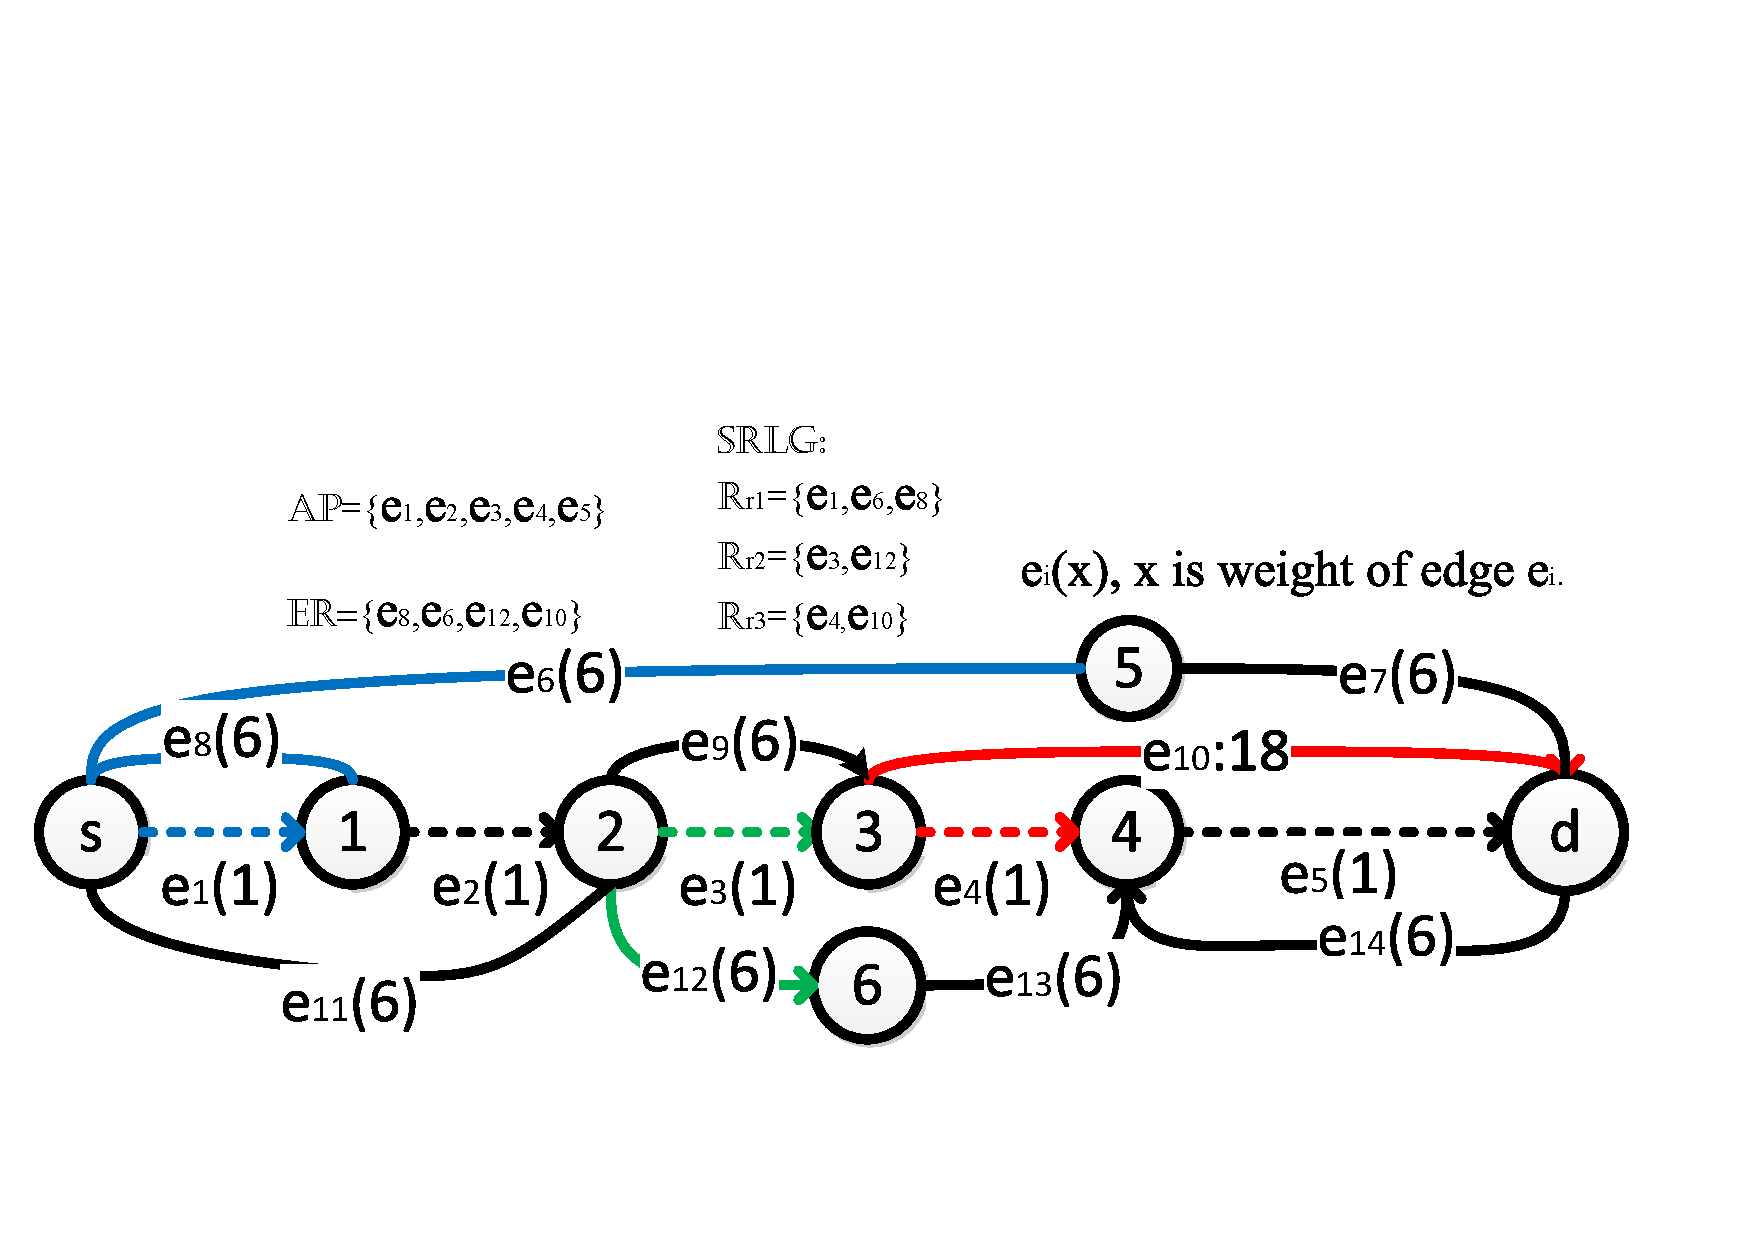
\includegraphics[width=4.35in]{franz/SampleTwoInitGraph}
%\caption{Shortest weight AP in a network graph with star-style SRLG}\label{fig:SampleTwoInitGraph}
%\end{figure*}
%\begin{figure*}[tp]
%\centering
%% Requires \usepackage{graphicx}
%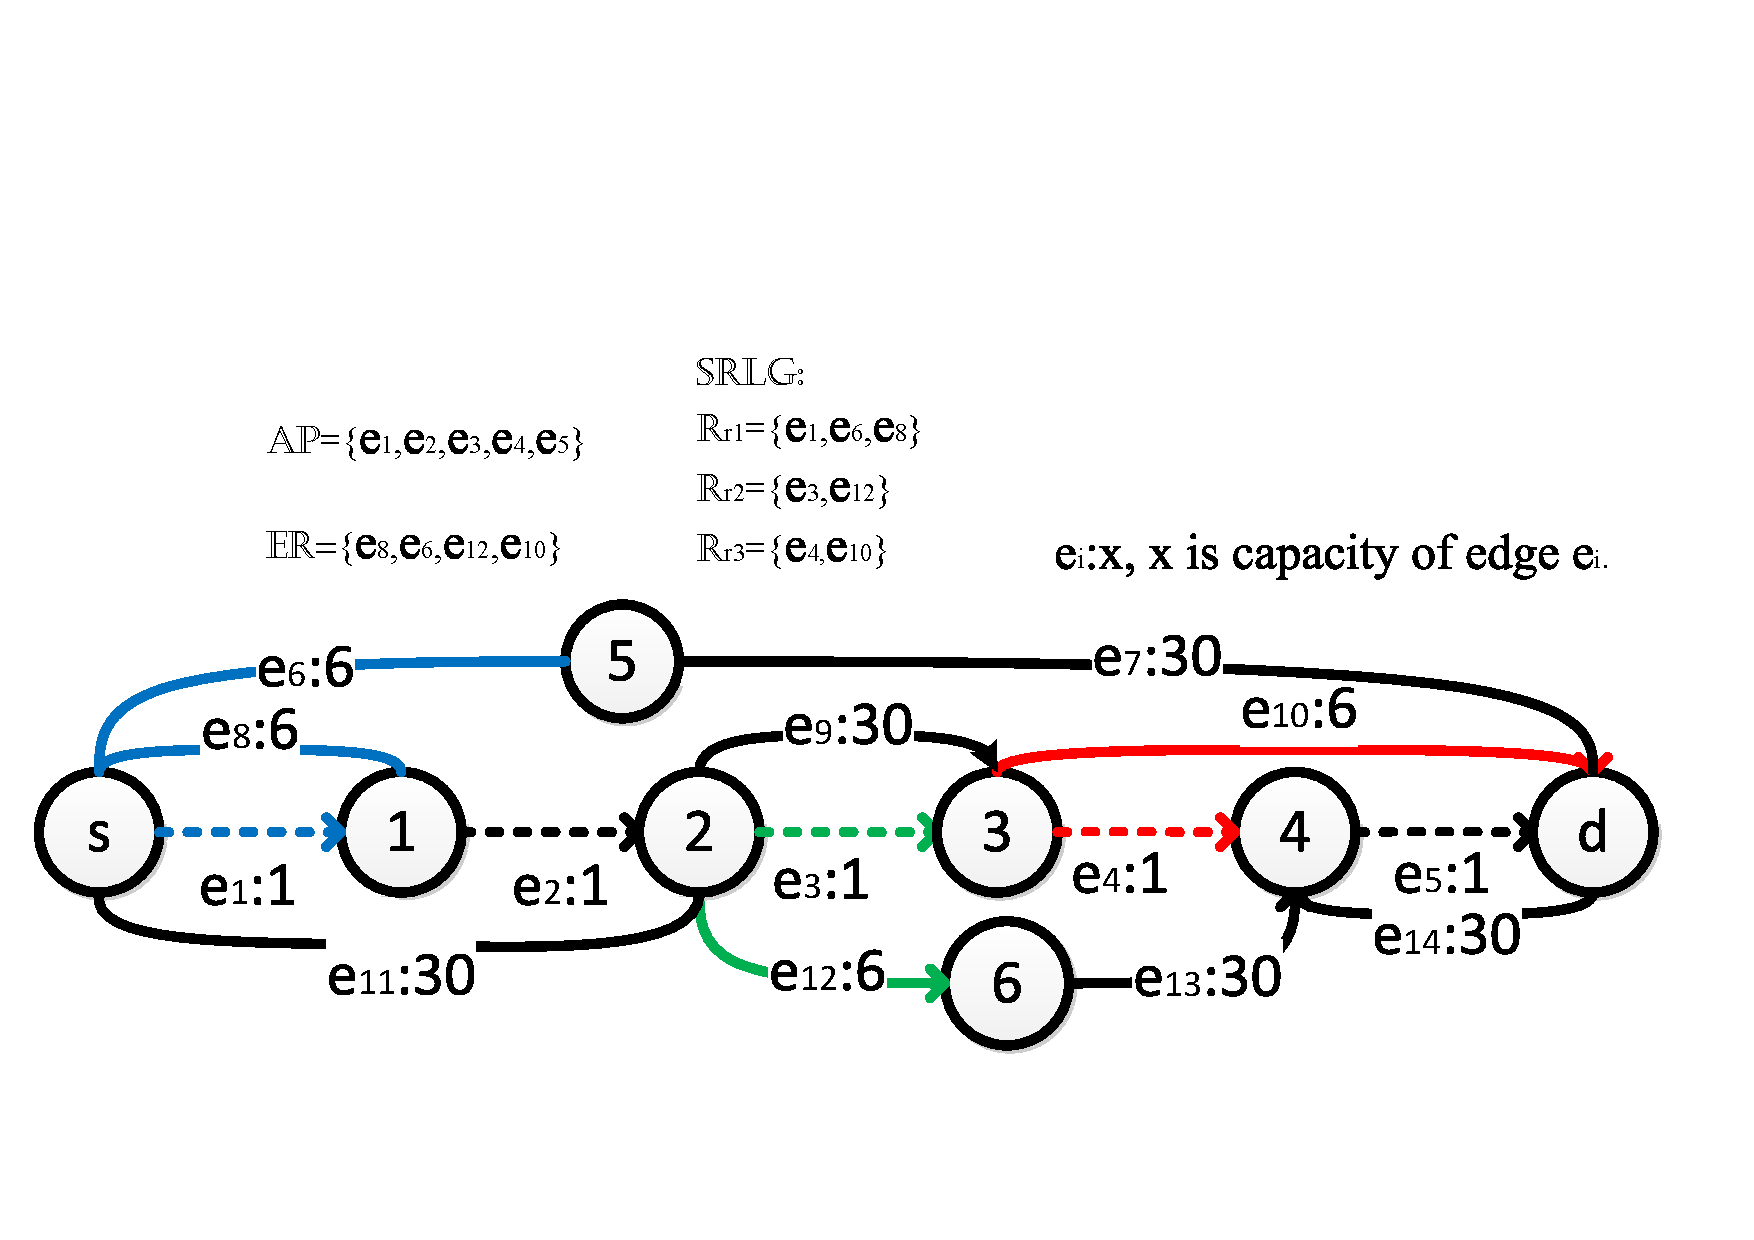
\includegraphics[width=4.35in]{franz/SampleTwoInitGraphFlowGraph}
%\caption{Network graph with star-style SRLG under well set capacity}\label{fig:SampleTwoInitGraphFlowGraph}
%\end{figure*}
%\begin{figure*}[tp]
%\centering
%% Requires \usepackage{graphicx}
%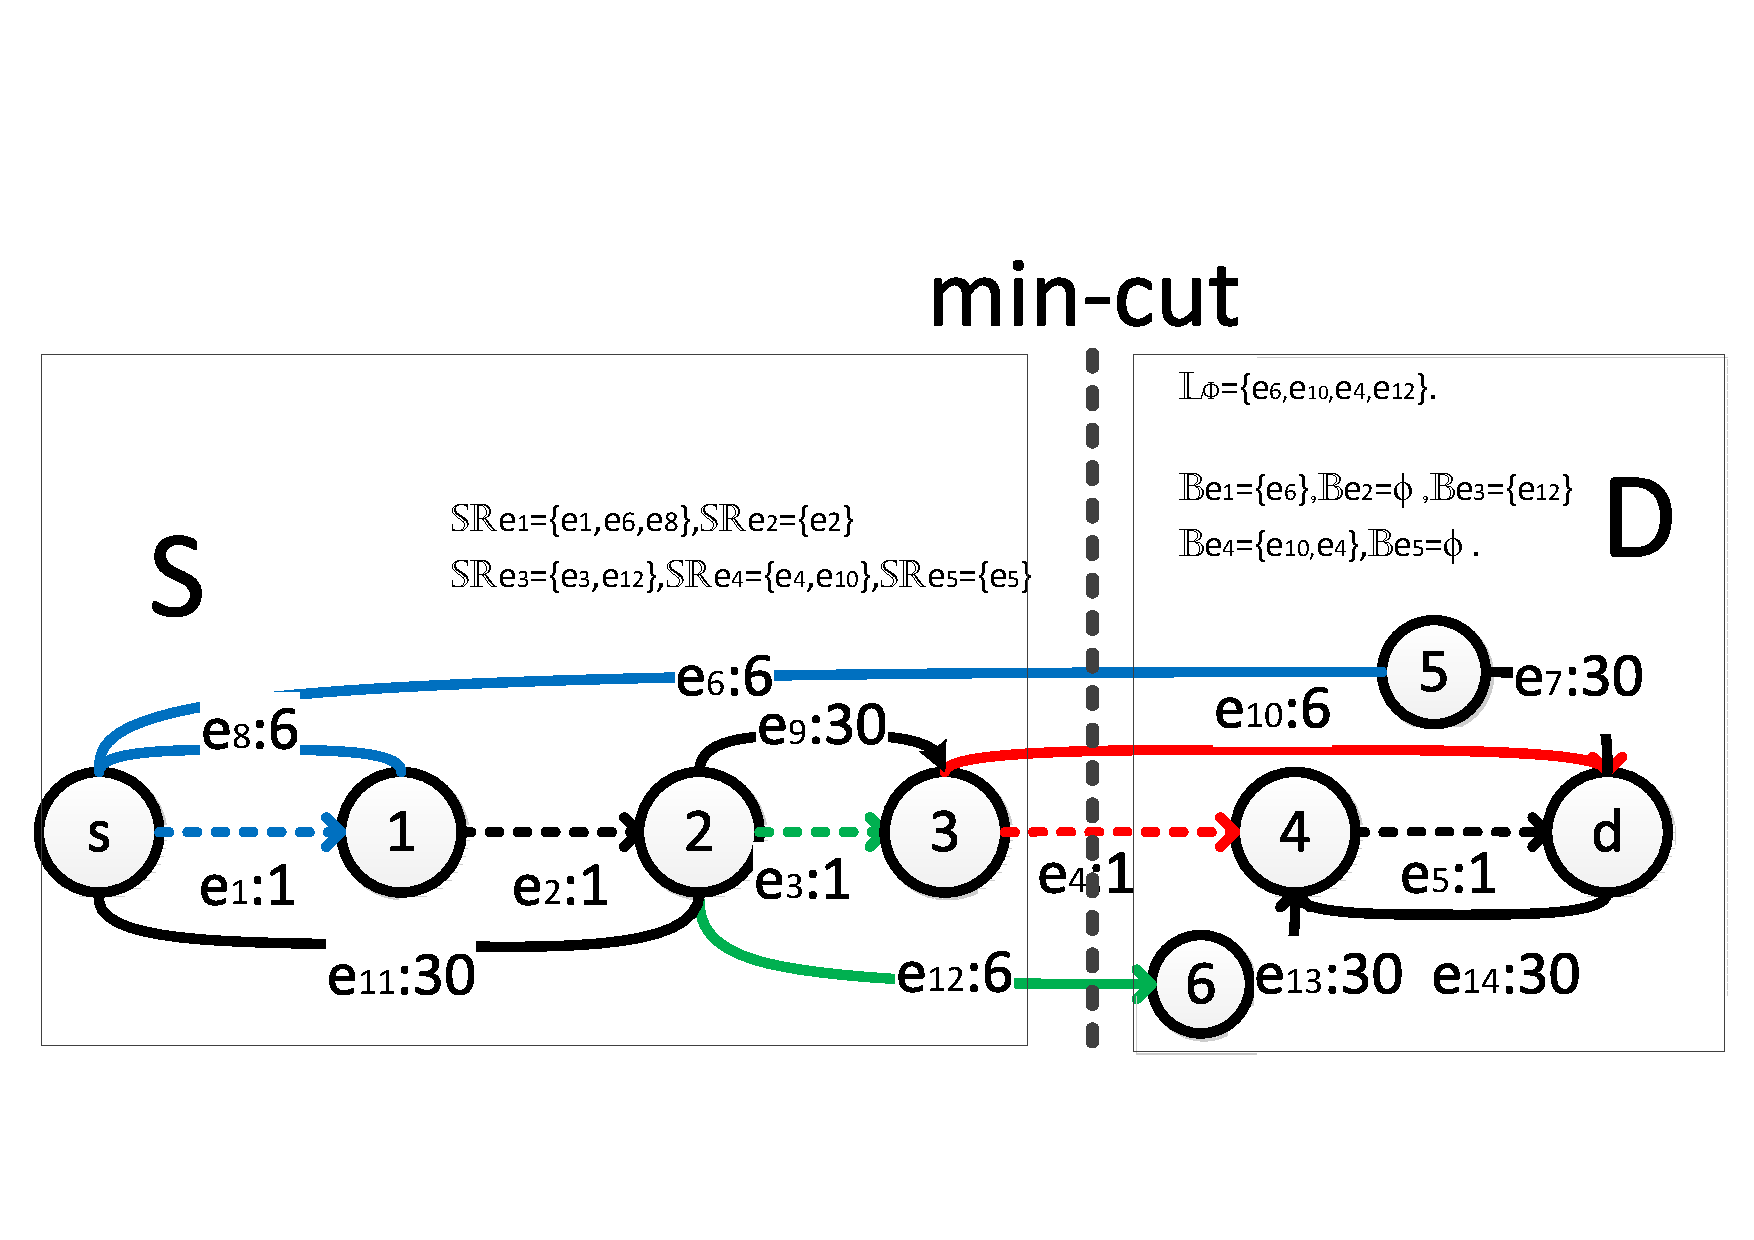
\includegraphics[width=4.35in]{franz/SampleTwoInitGraphCutGraph}
%  \caption{Min cut in the network graph with star-style SRLG, $\mathbb{SR}_{e_1}=\{e_1,e_6,e_8\},\mathbb{SR}_{e_2}=\{e_2\},\mathbb{SR}_{e_3}=\{e_3, e_{12}\},\mathbb{SR}_{e_4}=\{e_4, e_{10}\},\mathbb{SR}_{e_5}=\{e_5\}. \mathbb{L}_{\Phi}=\{e_{6},e_{10},e_{4},e_{12}\}. \mathbb{B}_{e_1}=\{e_6\},\mathbb{B}_{e_2}=\emptyset,\mathbb{B}_{e_3}=\{e_{12}\},\mathbb{B}_{e_4}=\{e_{10},e_4\}, \mathbb{B}_{e_5}=\emptyset$.}\label{fig:SampleTwoInitGraphCutGraph}
%\end{figure*}



%\begin{figure*}[tp]
%  \centering
%  % Requires \usepackage{graphicx}
%  \includegraphics[width=4.35in]{franz/MultiSRLGGraph}
%  \caption{when every link belong more than one SRLG, suppose $R_{e_3}=\{R_2,R_3\},R_{e_4}=\{R_1\},R_{e_5}=\{R_3\},R_{e_{11}}=\{R_1,R_2\},R_{e_{13}}=\{R_2,R_3\},R_{e_{19}}=\{R_1,R_3\}$. $SR_3=\{e_5,e_{11},e_{13},e_{19}\},SR_4=\{e_{11},e_{19}\},SR_5=\{e_3,e_{13},e_{19}\},SR_6=\emptyset,$ and other $SR_i=\emptyset$. $\mathbb{L}=\{e_{11},e_{13},e_6,e_{19}\}$. $B_3=\{e_{11},e_{13},e_{19}\},B_4=\{e_{11},e_{13}\},B_5=\{e_{13},e_{19}\},B_6=\{e_{6}\}$, other $B_i=\emptyset$}\label{fig:MultiSRLGGraph}
%\end{figure*}
%
%given an input $\left( {L_{\Phi},{B_{{e_1}}},{B_{{e_2}}}, \cdots ,{B_{{e_{|AP|}}}}} \right)$ of the set cover problem, we introduce a variable $x_{e_i}$ for block set $B_{e_i}$, with the intended meaning that $x_{e_i} = 1$ when $B_{e_i}$ is selected,
%and $x_{e_i} = 0$ otherwise. We can express the set cover problem as the following integer linear program:
%\begin{equation}
%\begin{array}{l}
% minimize\ {\rm{    }}\sum\limits_{i = 1}^{\left| AP \right|} {{x_i}}  \\
% subject\ to{\rm{    }} \cup _{i = 1}^{\left| AP \right|}{x_i}{B_i} \supseteq \mathbb{L} \\
% {\rm{                }}{x_i} \in \{ 0,1\}  \\
% \end{array}
% \label{eq:cover problem}
%\end{equation}
%As problem in (\ref{eq:cover problem}) is an integer linear program which is usually an NP-hard problem with its complexity depends on the $|AP|$.
%
%To efficiently solve problem in (\ref{eq:cover problem}), we apply relaxation technique to transform the original NP-hard optimization problem in (\ref{eq:cover problem}) into a linear programme (\ref{equ:relaxILP}) by replacing the integer constraint from ${x_i} \in \{ 0,1\}$ to $0\leq x\leq 1$.
%\begin{equation}
%\begin{array}{l}
% minimize\ {\rm{    }}\sum\limits_{i = 1}^{\left|AP \right|} {{x_i}}  \\
% subject\ to{\rm{    }} \cup _{i = 1}^{\left| \mathbb{L} \right|}{x_i}{B_i} \supseteq \mathbb{L} \\
% {\rm{                }}{0\leq x_i\leq 1}  \\
% \end{array}
%\label{equ:relaxILP}
%\end{equation}
%
%, that can be solvable in polynomial time.
%we solve the linear programming relaxation Equ(\ref{equ:relaxILP}), and we find an optimal fractional solution $x^*$
%to the relaxation, that is, we are given a number $x^*_i$ in the range $[0, 1]$ for every set $B_i$. the next most natural approach after rounding the $x_i^*$ to the nearest integer is to think of each $x_i^*$ as a probability, and we can think of the solution $x^*$ as describing
%a probability distribution over ways of choosing some of the subsets $B_1,B_2,\ldots,B_{|AP|}$, in which we choose $B_1$ with probability $x_1^*$, $B_2$ with probability $x_i^*$, and so on.
%
%\begin{algorithm}
%\caption{Select x}
%\label{alg:min-min}
%\begin{algorithmic}[1]
%\REQUIRE
%$x_1,x_2,\ldots,x_{|\mathbb{L}|}$ \\
%$B_1,B_2,\ldots,B_{|\mathbb{L}|}$\\
%$\mathbb{L}$
%\ENSURE
%$CSLS$
%\STATE $CSLS\leftarrow \emptyset$
%\STATE $B\leftarrow \emptyset$
%\FOR{$1\leq i\leq |AP|$}
%\STATE{select the i-th lagest value of $x$: $x_j$}
%\STATE $B\leftarrow B\cup B_j$
%\STATE $CSLS\leftarrow CSLS\cup e_j$
%\IF{$|B|=|\mathbb{L}|$}
%\RETURN $CSLS$
%\ENDIF
%\ENDFOR
%\end{algorithmic}
%\end{algorithm}
